 \documentclass[UTF8]{ctexart}
    \title{程序报告2}
    \author{Charles Shen}
    \date{\today}
    \begin{document}
    \maketitle
    \section{问题分析}
    \paragraph{}
    读入两个正整数,输出其最大公约数和最小公倍数,验证结果正确性并输出时间。
    这个问题可以拆分为五个模块:读入两个正整数,计算最大公约和最小公倍数,计时,随机样例生成和验证,输出。
    \section{程序实现}
    \paragraph{读入正整数}
    这个模块我调用了上次作业中加入代码构件库的判断并读入正整数模块(cp\_integer.cpp和.h),重复2次执行。由于上次作业中已经验证其正确性,这次不再验证。
    \paragraph{计算最大公约数和最小公倍数}
    这个模块我用一个类cp\_two\_integers实现( 具体代码在同名.h和.cpp文件中,已加入代码构件库) 。
    \subparagraph{}
    算法思想:求最大公约数$GCD$用辗转相除法,最小公倍数$LCM$则在求出最大公约数$GCD$后用公式$LCM=a*b/GCD$求出。求最大公约数代码如下:
     \begin{figure}[htbp]
    	\centering
    	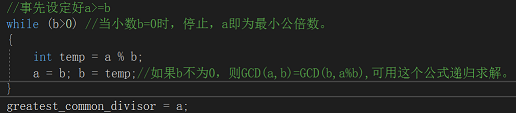
\includegraphics{a1.png}
    	\caption{求最小公倍数和最大公约数代码}
    \end{figure}
    \subparagraph{}
    程序验证:验证了五组数据:相等,a整除b,b整除a,一般情况,大数。验证结果如下。
    \begin{figure}[htbp]
   	\centering
   	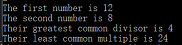
\includegraphics{b1.png}
   	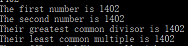
\includegraphics{b2.png}
   	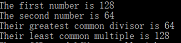
\includegraphics{b3.png}
   	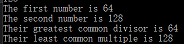
\includegraphics{b4.png}
   	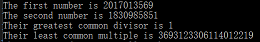
\includegraphics{b5.png}
   	\caption{测试数据及结果}
   \end{figure}
    \paragraph{计时}
    这个模块我参考了课件里的程序,建立一个类cp\_time\_by\_clock(代码在同名.cpp和.h文件里,已加入代码构件库),存储开始时间,结束时间。
    用clock函数获取开始时间和结束时间,并且借助CLOCKS\_PER\_SEC求出具体时间。  
    \paragraph{验证}
    这个模块基本思路是按照最大公约数和最小公倍数定义。当两者均为正整数,并且最大公约数为公约数,最小公倍数为公倍数,没有比最大公约数大的公约数,没有比最小公倍数小的公倍数才成立。
    验证几万组机器生成的随机数据后再输出结果。具体代码如下:
     \begin{figure}[htbp]
    	\centering
    	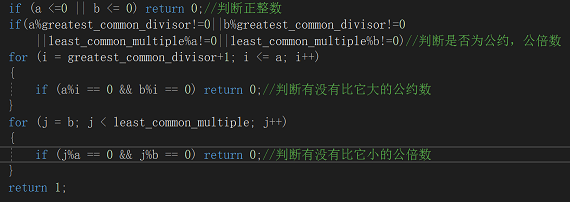
\includegraphics{c.png}
    	\caption{程序自动验证代码}
    \end{figure}
    \paragraph{输出}
    输出部分集中在main文件里。验证结果如下:
    \begin{figure}[htbp]
    	\centering
    	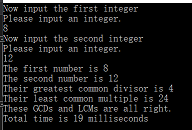
\includegraphics{d1.png}
    	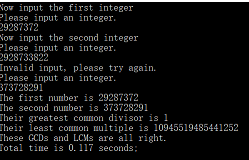
\includegraphics{d2.png}
    	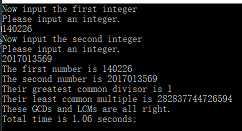
\includegraphics{d3.png}
    	\caption{测试数据及结果}
    \end{figure}
    \section{评价}
    程序对可能的bug进行了规避(包括读入bug,最小公倍数溢出等问题),而且采用辗转相除算法求解问题,提高了运行效率,同时能机器生成随机数自动验证。
    \end{document}